\documentclass[a4paper]{article}
\usepackage[top=1in, bottom=1.25in, left=1.25in, right=1.25in]{geometry}
\usepackage{amsmath}
\usepackage{multicol}
\usepackage{graphicx}
\RequirePackage{ltxcmds}[2010/12/07]
%opening
\title{Pulse Shaper}

\begin{document}

\maketitle

This block applies a raised-cosine filter to the signal. It accepts one input signal that is a sequence of Dirac delta functions and it produces one output signal continuous in time and in amplitude.

\subsection*{Input Parameters}

\begin{itemize}
	\item filterType\{RaisedCosine\} \linebreak
	\item impulseResponseTimeLength\{16\}\linebreak (int) 
	\linebreak (This parameter is given in units of symbol period)
	\item rollOfFactor\{0.9\} \linebreak
	(real $\in$ [0,1])
\end{itemize}

\subsection*{Methods}

PulseShaper(vector$<$Signal *$>$ \&InputSig, vector$<$Signal *$>$ OutputSig) :FIR$\_$Filter(InputSig, OutputSig)\{\};
\bigbreak	
void initialize(void);
\bigbreak	
void setImpulseResponseTimeLength(int impResponseTimeLength)\{ impulseResponseTimeLength = impResponseTimeLength; \};
\bigbreak
int const getImpulseResponseTimeLength(void) \{ return impulseResponseTimeLength; \};
\bigbreak	
void setFilterType(PulseShaperFilter fType)\{ filterType = fType; \};
\bigbreak
PulseShaperFilter const getFilterType(void)\{ return filterType; \};
\bigbreak	
void setRollOffFactor(double rOffFactor)\{ rollOffFactor = rOffFactor; \};
\bigbreak
double const getRollOffFactor()\{ return rollOffFactor; \};

\subsection*{Functional Description}

The filter's transfer function is defined by the vector \textit{impulseResponse}. The parameter \textit{rollOfFactor} is a characterisitic of the filter and is used to define its transfer function.

\subsection*{Input Signals}

\subparagraph*{Number}: 1

\subparagraph*{Type}: Sequence of Dirac Delta functions (ContinuousTimeDiscreteAmplitude)

\subsection*{Output Signals}

\subparagraph*{Number}: 1

\subparagraph*{Type}: Sequence of impulses modulated by the filter (ContinuousTimeContinuousAmplitude)

\subsection*{Example}

\begin{figure}[h]
	\centering
	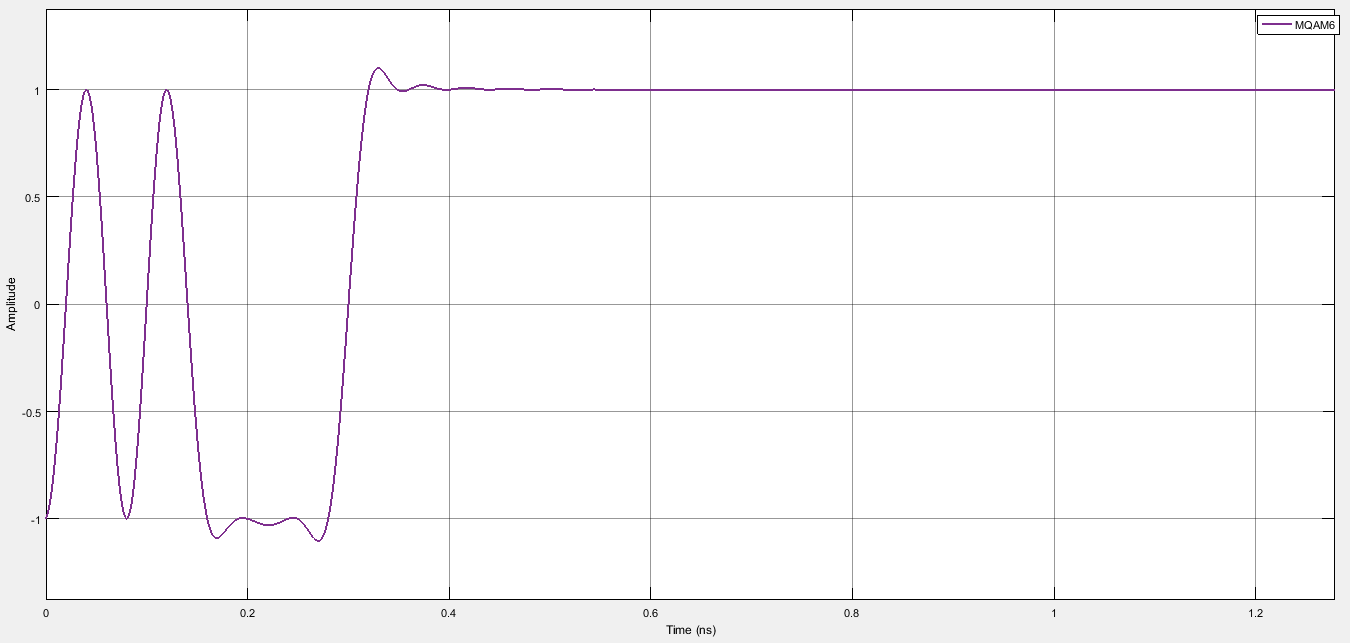
\includegraphics[width=\textwidth]{MQAM6_DeterministicAppendZeros}
	\label{MQAM6_DeterministicAppendZeros}\caption{Example of a signal generated by this block for the initial binary signal "0100011101010101"}
\end{figure}

\subsection*{Sugestions for future improvement}

Include other types of filters.

\end{document}